\documentclass[10pt,twocolumn]{article}
\usepackage{graphicx}
\usepackage[margin=0.5in]{geometry}
\usepackage[cmex10]{amsmath}
\usepackage{array}
\usepackage{booktabs}
\usepackage{mathtools}
\usepackage[parfill]{parskip}
\title{\textbf{Optimization Assignment}}
\author{Divya Sai-FWC22094}
\providecommand{\norm}[1]{\left\lVert#1\right\rVert}
\providecommand{\abs}[1]{\left\vert#1\right\vert}
\let\vec\mathbf
\newcommand{\myvec}[1]{\ensuremath{\begin{pmatrix}#1\end{pmatrix}}}
\newcommand{\mydet}[1]{\ensuremath{\begin{vmatrix}#1\end{vmatrix}}}
\providecommand{\brak}[1]{\ensuremath{\left(#1\right)}}
\providecommand{\lbrak}[1]{\ensuremath{\left(#1\right.}}
\providecommand{\rbrak}[1]{\ensuremath{\left.#1\right)}}
\providecommand{\sbrak}[1]{\ensuremath{{}\left[#1\right]}}

\begin{document}

\maketitle

\textbf{\large{Problem Statement: }} \\
\raggedright Let P be a variable point on the ellipse $$\frac{x^2}{a^2}+ \frac{y^2}{b^2} = 1 $$ with foci $F_1$ and $F_2$. If A is the area of the triangle $PF_1$ $F_2$ then the maximum value of A is

\textbf{To Find:} The maximum area of the triangle.

\textbf{Given:} Ellipse with foci $F_1$ anf $F_2$.\\
\section{Solution}
The equation of the ellipse
\begin{align}
	\vec{x}^T\vec{V}\vec{x} + f = 0 
	\label{eq:ellipse}	
\end{align}
where,
\begin{align}
	\vec{V} = \myvec{b^2&0\\0&a^2}
	\\f = -a^2b^2
\end{align}
	\begin{align}
		\myvec{0&1}\vec{x} = \vec{0}
	\end{align}
\\Given variable point P. let,vertex be $(x,y)$
\\Given $F_1$ and $F_2$ are the foci of the ellipse.
\begin{align}
	\vec{P} = \myvec{x \\ y} ;
	\vec{F_1} = \myvec{ae \\ 0} ;
	\vec{F_2} = \myvec{-ae \\ 0} 
\end{align}
\textbf{The area A of the triangle $PF_1$ $F_2$ is given by }
	
\begin{align}
A = \frac{1}{2} \mydet{\vec{\brak{P-F_1}} \times \vec{\brak{P-F_2}}}
	\\ \implies \frac{1}{2} \mydet{x-ae & x+ae \\ y & y}	
\end{align}
\begin{center}	
	\boxed{ A = yae}
\end{center}
from equation of ellipse,
\begin{align}
	 y = \frac{b}{a}\sqrt{a^2-x^2}
\end{align} 
\vspace{5mm}
Substitute eq(9) in eq(8),
\vspace{5mm}
\begin{align}
 A=abe \sqrt{1-\frac{x^2}{a^2}}
\end{align}

\textbf{Objective function:}
\begin{align}
A=\max_x abe \sqrt{1-\frac{x^2}{a^2}}
\end{align}

\textbf{constraints:}\\
\begin{center}
a$>$0\\b$>$0\\x$>$0
\end{center}
Let the length of major and minor axis of the ellipse be 3,1
\begin{align}
	a = 3
	\\b=1
\end{align}
\section{Calculation of Maxima using gradient ascent algorithm}
The maximum area of the triangle will be found by finding the local maxima of the function.
Using gradient ascent method we can find its maxima ,
    \begin{align}
        x_{n+1} &= x_n + \alpha \nabla A \\
	    \implies x_{n+1} &= x_n + \alpha \brak{\frac{-ebx}{\sqrt{a^2-x^2}}}
    \end{align}

where \\
\begin{enumerate}
\item $\alpha$ = 0.001
\item $x_{n+1}$ is current value
\item $x_{n}$ is previous value
\item precession = 0.00000001
\item maximum iterations = 100000000
\end{enumerate}
\begin{align}
        \boxed{\text{Maxima} = 2.8284}\\
        \boxed{\text{Maxima Point} = 0.0000}
        \end{align}

\section{Result}
   \begin{center}
  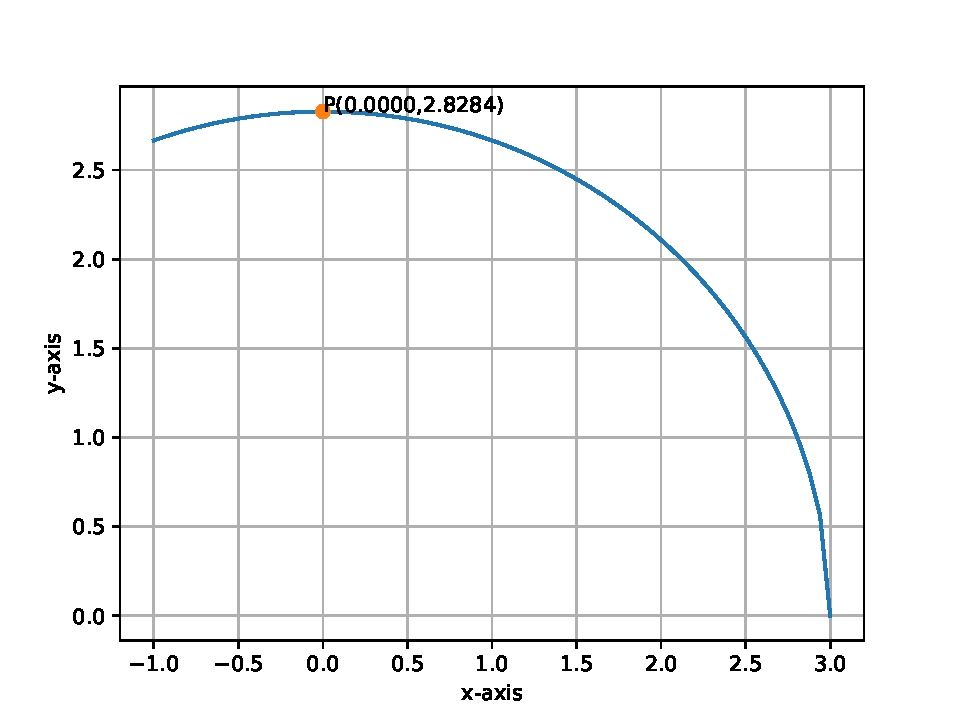
\includegraphics[scale=0.5]{opti.pdf}
    \end{center}
\end{document}